\chapter{数字签名与身份认证}

\question{计算机安全的四大原则},机密性、完整性、可认证性、不可抵赖性。

\question{安全协议}
\begin{enumerate}
	\item 以密码学为基础
	\item 也是通信协议
\end{enumerate}
分类:
\begin{enumerate}
	\item 密钥生成协议
	\item 认证协议
	\item 电子商务协议
	\item 安全多方计算协议
\end{enumerate}

\question{数字签名},\textbf{基于非对称密码算法},是一串数据,该数据仅能由签名人生成,并且该数据能够表明签名人的身份。一般由两个部分组成
\begin{enumerate}
	\item 签名算法,由签名方秘密保存
	\item 验证算法,通常是公开的,便于他人验证签名的有效性
\end{enumerate}
通常分为两类:
\begin{enumerate}
	\item 直接数字签名
	\item 基于仲裁的数字签名
\end{enumerate}

\question{数字签名算法}
\begin{enumerate}
	\item DSA
	\begin{figure}[H]
		\centering
		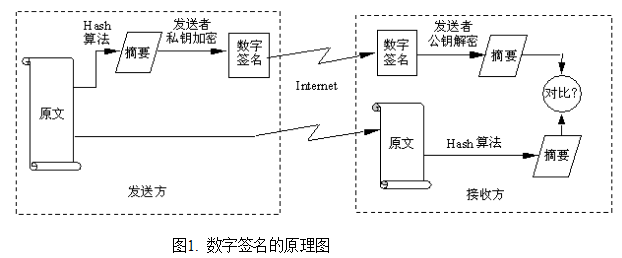
\includegraphics[width=0.7\linewidth]{dsa.png}
	\end{figure}
	\begin{enumerate}
		\item 使用SHA编码将发送文件加密产生128bit的数字摘要; 
		\item 发送方用自己的专用密钥对摘要再加密,形成数字签名; 
		\item 将原文和加密的摘要同时传给对方; 
		\item 接受方用发送方的公共密钥对摘要解密,同时对收到的文件用SHA编码加密产生同一摘要; 
		\item 将解密后的摘要和收到的文件在接受方重新加密产生的摘要相互对比,如果两者一致,则说明在传送过程中信息没有破坏和篡改。否则,则说明信息已经失去安全性和保密性。
	\end{enumerate}
\end{enumerate}